\chapter{Results}
\label{sec:results}
The results of the developed algorithms will be presented in this chapter. The mentioned programs and functions can be found on the provided CD.   

\section{RRT* Path Planning in 2D}

In this section, the results of the path curvature evaluation on the 2D plane are discussed. In the cost function, one considers euclidean distances on the one hand and angular changes on the other. A cost function consisting of a combination of both attributes does not bring any benefits and therefore was not considered. The m-file \verb+RRTstar_Obstacles_2D.m+ in the folder \verb|Curvature_Evaluation| is used and the following parameters are chosen:

\begin{itemize}
	\item
	$10 \times 9.5$ map
	\item
	$x_{initial}=4.75$ and $y_{initial}=2.75$
	\item
	$x_{initial\_parent}=5$ and $y_{initial\_parent}=2.75$ \footnote{These additional variables are needed to define the heading in the initial configuration}
	\item
	$x_{final}=4.75$ and $y_{final}=6.75$ 
	\item 
	$\gamma_{RRT^{*}}=10$
	\item
	$\eta=1$
	\item
	$iteration=50'000$
\end{itemize} 

\subsection{Cost Function: Considering Euclidean Distance}
\label{sec:euclidean}

\begin{itemize}
	\item
	$w_{1}=1$ and $w_{2}=0$
	\item
	$140\,s$ to complete the calculation.
\end{itemize} 

As one can see in Figure \ref{pics:RRTstar_w1}, the RRT* algorithm calculates a path, which follows mostly the edges of the obstacles. By inflating the obstacles in the order of the radius of \textit{Scubo}, one can create buffer zones for the robot to move without hitting obstacles. Furthermore, the path takes sharp turns at edges. This is also not a problem for the real system, since the robot is omnidirectional and is able to move in any direction without prior change of its orientation.

\begin{figure} [h]
	\centering
	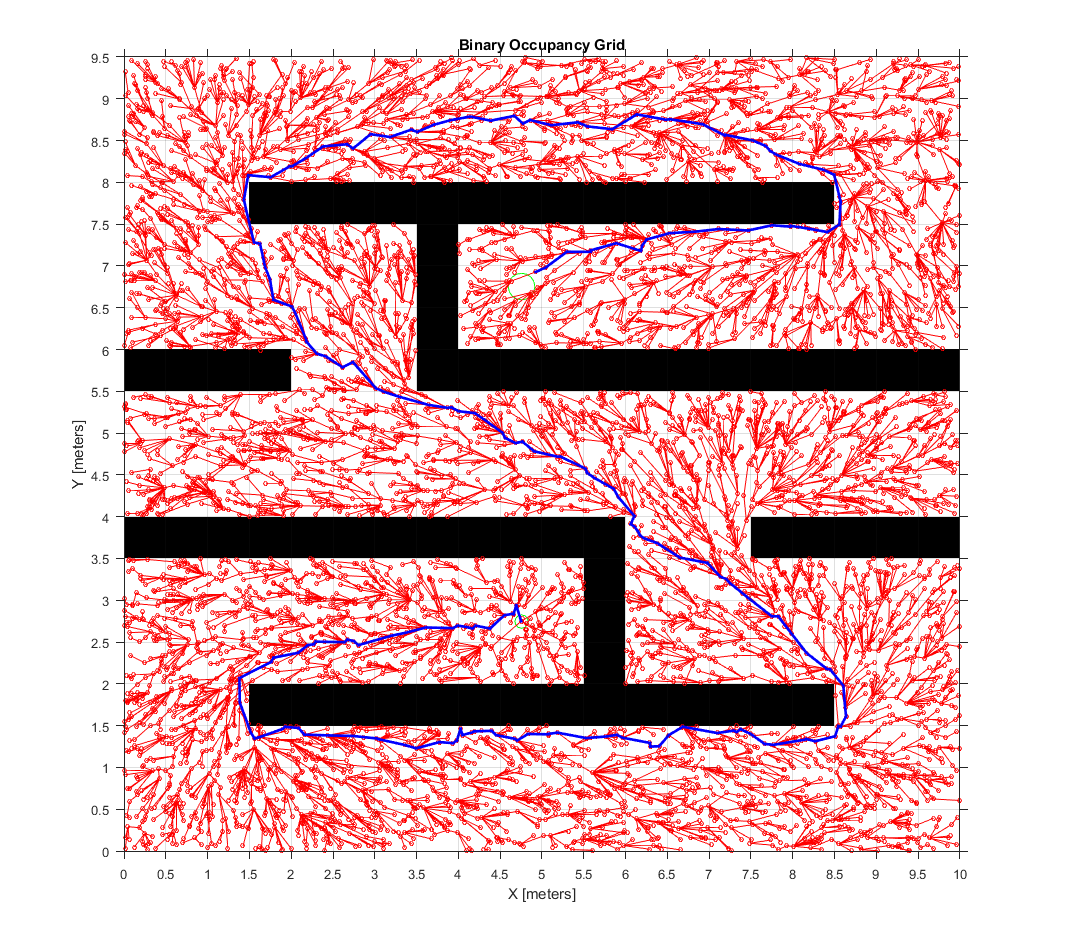
\includegraphics[width=1\textwidth]{images/RRTstar_w1.png}
	\caption{2D RRT* Path: Considering euclidean distance in the cost function.}
	\label{pics:RRTstar_w1}
\end{figure}


\subsection{Cost Function: Considering Angular Change}

\begin{itemize}
	\item
	$w_{1}=0$ and $w_{2}=1$
	\item
	$102\,s$ to complete the calculation.
\end{itemize}

As expected, a much smoother path can be generated under the same condition by considering the angular change in the cost function (see Figure  \ref{pics:RRTstar_w2}). Surprisingly, this task takes less time to compute than the one described in the previous Section  \ref{sec:euclidean}.

\begin{figure} [h]
	\centering
	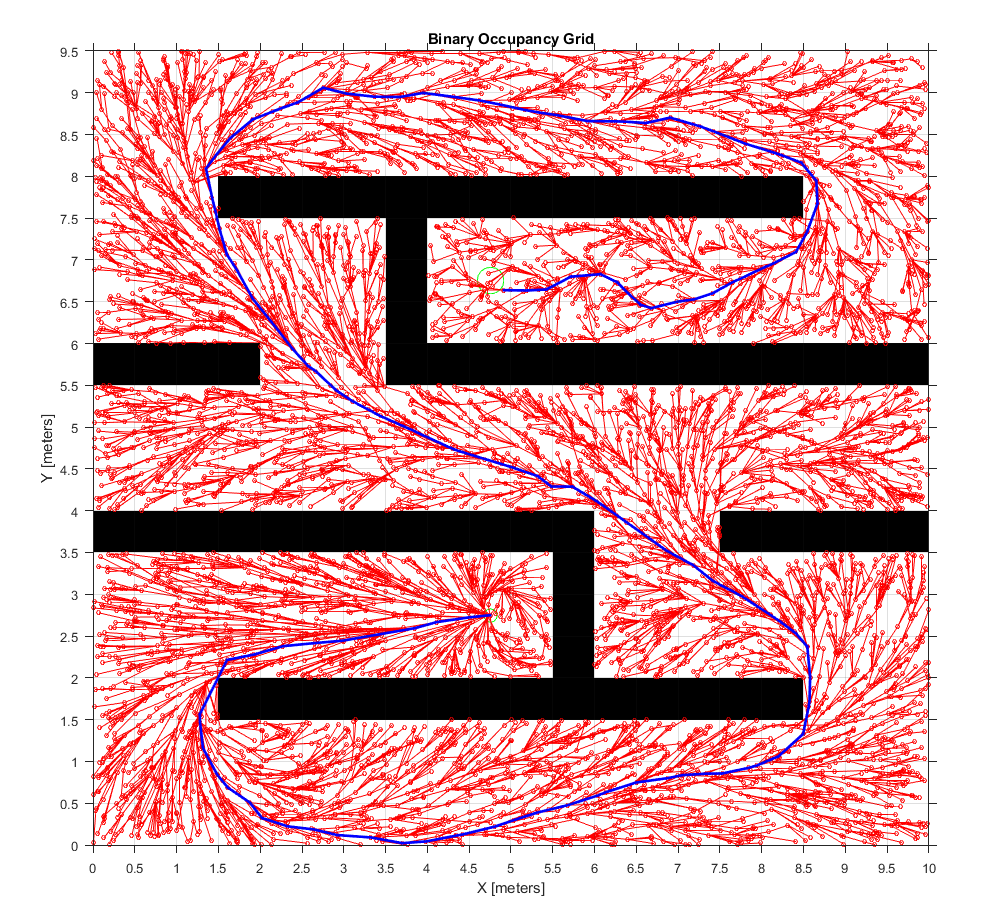
\includegraphics[width=1\textwidth]{images/RRTstar_w2.png}
	\caption{2D RRT* Path: Considering angular change in the cost function.}
	\label{pics:RRTstar_w2}
\end{figure}

\section{RRT* Path Planning in 3D}

The visualization in 3D is done with \textit{Paraview}. The m-file \verb+RRTstar_Obstacles_3D.m+ is used to generate the map, the states and the resulting paths. With \verb+VtkWriter.m+, the results are transformed into VTK-format in order to display it in \textit{Paraview}. The following parameters are chosen:

\begin{itemize}
	\item
	$10 \times 10 \times 10$ map
	\item
	$x_{initial}=1$, $y_{initial}=1$ and $z_{initial}=1$
	\item
	$x_{final}=1$, $y_{final}=1$ and $z_{final}=9$
	\item 
	$\gamma_{RRT^{*}}=10$
	\item
	$\eta=2$
	\item
	$iteration=1000$
\end{itemize}

As one can see in Figure \ref{pics:rrstar_3d}, the generated path in 3D is feasible. The red wall is an obstacle with a hole in the middle. The algorithm is able to find a path between start and goal through the obstacle.

\begin{figure} [h]
	\centering
	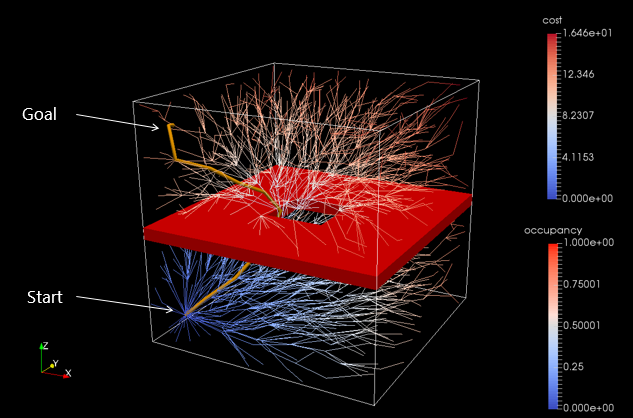
\includegraphics[width=1\textwidth]{images/rrtstar_3d.png}
	\caption{3D RRT* Path}
	\label{pics:rrstar_3d}
\end{figure}

\section{Object Scanning}
\label{sec:object_scanning}

For object scanning, the following files were used. Point cloud datas were stored in \verb+coral.vtr+. The file \verb|occupancy_calculation.m| calculates the occupancy matrix regarding Formulas \ref{eq:occupancy}, \ref{eq:transformation} and \ref{eq:transformation_occupancy}. The viewpoints are set in \verb|view_states_calculation.m| and the corresponding cost matrix and the possible paths between all viewpoints is computed in \verb|traveling_salesman_cost.m|. The order of the viewpoints can be defined in two ways. The file \verb|ts_greedy_algorithm.m| sets the order according the greedy algorithm. For a order by the LKH algorithm, one can use the file \verb|compute_traveling_salesman.m| with the corresponding executables\footnote{http://webhotel4.ruc.dk/~keld/research/LKH/}.  

\subsection{Route by Greedy Algorithm}

As expected, the route generated by the greedy algorithm is not efficient, since the path go over the object two times (see Figure \ref{pics:greedy}).

\begin{figure} [h]
	\centering
	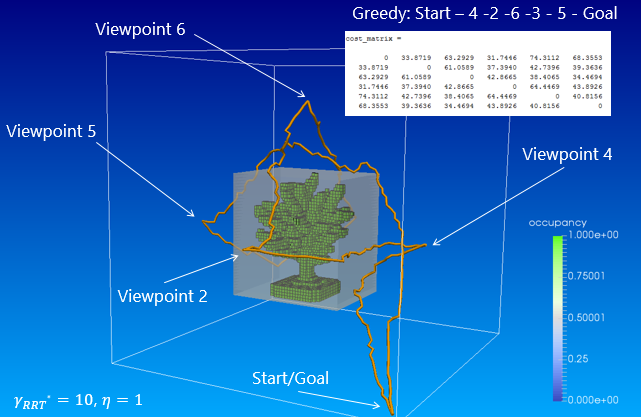
\includegraphics[width=1\textwidth]{images/greedy.png}
	\caption{Object scanning route according greedy algorithm.}
	\label{pics:greedy}
\end{figure}

\subsection{Route by LKH Algorithm}

A much more efficient route can be generated by using the LKH algorithm. The path goes around the object in a reasonable manner and ends in the starting configuration (see Figure \ref{pics:lkh_route}).

\begin{figure} [h]
	\centering
	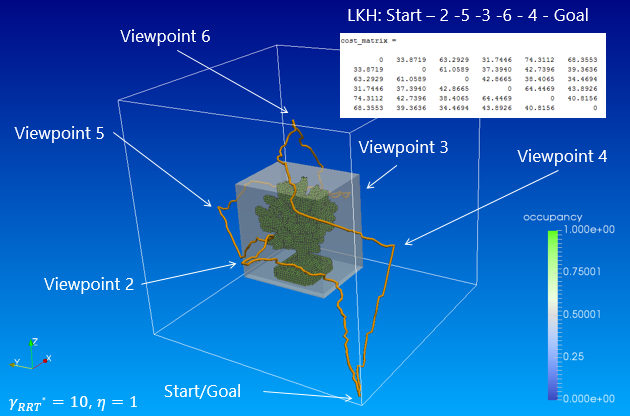
\includegraphics[width=1\textwidth]{images/lkh_route.png}
	\caption{Object scanning route according the LKH algorithm.}
	\label{pics:lkh_route}
\end{figure}